%==============================================================================
% Sjabloon onderzoeksvoorstel bachelorproef
%==============================================================================
% Gebaseerd op LaTeX-sjabloon ‘Stylish Article’ (zie voorstel.cls)
% Auteur: Jens Buysse, Bert Van Vreckem
%
% Compileren in TeXstudio:
%
% - Zorg dat Biber de bibliografie compileert (en niet Biblatex)
%   Options > Configure > Build > Default Bibliography Tool: "txs:///biber"
% - F5 om te compileren en het resultaat te bekijken.
% - Als de bibliografie niet zichtbaar is, probeer dan F5 - F8 - F5
%   Met F8 compileer je de bibliografie apart.
%
% Als je JabRef gebruikt voor het bijhouden van de bibliografie, zorg dan
% dat je in ``biblatex''-modus opslaat: File > Switch to BibLaTeX mode.

\documentclass{voorstel}

\usepackage{lipsum}

%------------------------------------------------------------------------------
% Metadata over het voorstel
%------------------------------------------------------------------------------

%---------- Titel & auteur ----------------------------------------------------

% TODO: geef werktitel van je eigen voorstel op
\PaperTitle{Image recognition met Google Cloud AutoML}
\PaperType{Onderzoeksvoorstel Bachelorproef 2019-2020} % Type document

% TODO: vul je eigen naam in als auteur, geef ook je emailadres mee!
\Authors{Robbe Decorte\textsuperscript{1}} % Authors
\CoPromotor{Kenny Helsens\textsuperscript{2} (In The Pocket)}
\affiliation{\textbf{Contact:}
  \textsuperscript{1} \href{mailto:robbe.decorte@student.hogent.be}{robbe.decorte@student.hogent.be};
  \textsuperscript{2} \href{mailto:kenny.helsens@inthepocket.com}{kenny.helsens@inthepocket.com};
}

%---------- Abstract ----------------------------------------------------------

\Abstract{
Machine learning en AI zijn op dit moment een hot topic dat constant in verandering is. Op veel plaatsen
zoeken ze naar Data Scientists die een specifieke case bestuderen en een toegepast model trainen. Google
AutoML beweert deze stap grondig te vereenvoudigen, zodat iedereen met een basis machine learning kennis
een eigen model met interface kan produceren. Dus de vraag is als dit eerder een goed getimede marketing slogan van Google is of toch gerealiseerd kan worden in een bedrijfscontext. Dit wordt onderzocht door een eigen model te trainen en de correctheid ervan te verifiëren. Verder wordt onderzocht hoe zo'n complex systeem in elkaar zit alsook waar het zich bevindt tussen de traditionele manieren van werken. Een eerste blik bevestigt een goed werkend systeem maar het is niet duidelijk welke resultaten je bekomt voor de verschillende trainingsformules. Google Cloud AutoML is niet de eerste iteratie, er is telkens verder gebouwd uit vorige projecten waardoor de kans wel vergroot dat het naar de verwachtingen presteert.

\textbf{Perspectief} (Wat zegt de toekomst voor dit werk?).
}

%---------- Onderzoeksdomein en sleutelwoorden --------------------------------
% TODO: Sleutelwoorden:
%
% Het eerste sleutelwoord beschrijft het onderzoeksdomein. Je kan kiezen uit
% deze lijst:
%
% - Mobiele applicatieontwikkeling
% - Webapplicatieontwikkeling
% - Applicatieontwikkeling (andere)
% - Systeembeheer
% - Netwerkbeheer
% - Mainframe
% - E-business
% - Databanken en big data
% - Machineleertechnieken en kunstmatige intelligentie
% - Andere (specifieer)
%
% De andere sleutelwoorden zijn vrij te kiezen

\Keywords{Onderzoeksdomein. Machineleertechnieken en kunstmatige intelligentie --- Google --- Computer Vision} % Keywords
\newcommand{\keywordname}{Sleutelwoorden} % Defines the keywords heading name

%---------- Titel, inhoud -----------------------------------------------------

\begin{document}

\flushbottom % Makes all text pages the same height
\maketitle % Print the title and abstract box
\tableofcontents % Print the contents section
\thispagestyle{empty} % Removes page numbering from the first page

%------------------------------------------------------------------------------
% Hoofdtekst
%------------------------------------------------------------------------------

% De hoofdtekst van het voorstel zit in een apart bestand, zodat het makkelijk
% kan opgenomen worden in de bijlagen van de bachelorproef zelf.
%---------- Inleiding ---------------------------------------------------------

\section{Introductie} % The \section*{} command stops section numbering
\label{sec:introductie}

Machine learning en eenvoudig in dezelfde zin gebruiken, geen vanzelfsprekende opdracht maar wel iets dat Google probeert te realiseren. Met eigenschappen op hun site \autocite{Google2019} zoals: Uitstekende prestaties; Snel aan de slag; ontstaan er met Cloud AutoML toch enkele mogelijkheden om als programmeur (zonder professionele AI kennis) machine learning diensten te voorzien in een applicatie zonder dat er een data scientist bij het project betrokken wordt. Dit onderzoek, gefocust op het classificeren en herkennen van afbeeldingen, probeert aan te tonen dat deze service bruikbaar is voor bedrijven en hoe het scoort tegenover alternatieven.

%---------- Stand van zaken ---------------------------------------------------

\section{Literatuurstudie}
\label{sec:literatuurstudie}

% Voor literatuurverwijzingen zijn er twee belangrijke commando's:
% \autocite{KEY} => (Auteur, jaartal) Gebruik dit als de naam van de auteur
%   geen onderdeel is van de zin.
% \textcite{KEY} => Auteur (jaartal)  Gebruik dit als de auteursnaam wel een
%   functie heeft in de zin (bv. ``Uit onderzoek door Doll & Hill (1954) bleek
%   ...'')

Geautomatiseerde machine learning is het automatiseren van het trainingsproces bij een artificieel neuraal netwerk. De lage toegangsdrempel zorgt ervoor dat mensen met beperkte machine learning kennis sneller en simpeler een model kunnen trainen en gebruiken.

\subsection{Achterliggende werking}

\begin{figure}
    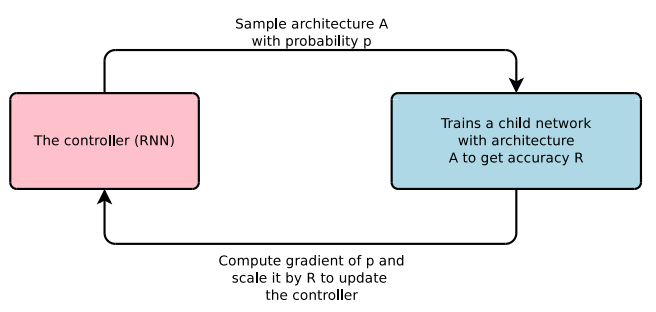
\includegraphics[width=\linewidth]{img/nas.png}
    \caption{Werking van Neural Architecture Search}
    \label{fig:nas}
\end{figure}

Dergelijke AutoML systemen gebruiken een techniek die het ontwerp van een artificieel neuraal netwerk kan automatiseren, beter bekend als Natural Architecture Search \autocite{Elsken2019}. Uit \textcite{ZophL2016} wordt vastgesteld dat deze techniek een gelijkaardige of zelfs betere performantie heeft dan modellen die door een ML-ingenieur ontworpen zijn.

Natural Architecture Search gebruikt Reinforcement Learning om een model te trainen. Deze manier van werken is fundamenteel anders dan gesuperviseerd / ongesuperviseerd leren omdat het model niet beter wordt door het gebruik van datasets. Als alternatief kan het neuraal netwerk beloningssignalen herkennen waardoor het kan leren welke acties leiden tot een positief resultaat \autocite{Lievens2019}.

Op figuur \ref{fig:nas} wordt gevisualiseerd hoe dit werkt. Op basis van controller structuur A (waarbij A een neuraal netwerk is) wordt een string met variabele lengte gegenereerd. Deze waarden worden gebruikt als parameters om een kind-netwerk aan te maken, die getraind wordt met echte data en waarbij de accuraatheid gemeten wordt aan de hand van een validatie dataset. Het resultaat wordt gebruikt als beloningssignaal voor de controller, bij de volgende iteratie kunnen er hogere kansen gegeven worden aan parameters die leiden tot accurate voorspellingen \autocite{ZophL2016}. De controller zijn zoekfunctie zal dus verbeteren over tijd.



\subsection{Gelijkaardige tools}
sdfq

%---------- Methodologie ------------------------------------------------------
\section{Methodologie}
\label{sec:methodologie}

Eerst en vooral wordt er een image dataset gemaakt die gebruikt wordt om de modellen te trainen en te valideren. Om een model te trainen is er een grote hoeveelheid data nodig. FFmpeg is een tool waarmee je de frames van een video (in dit geval een 360 graden video van het object) kan opsplitsen in afbeeldingen. De classificatie van de images wordt verwerkt met pandas, een data-analyse library voor Python.

Voor het experiment worden 2 modellen getraind met Google Cloud AutoML en AutoKeras. Zo kan het resultaat vergeleken worden met een open source alternatief. 

Er worden een aantal afbeeldingen geselecteerd van verschillende moeilijkheidsgraden om de modellen te toetsen.

%---------- Verwachte resultaten ----------------------------------------------
\section{Verwachte resultaten}
\label{sec:verwachte_resultaten}

\begin{figure}
    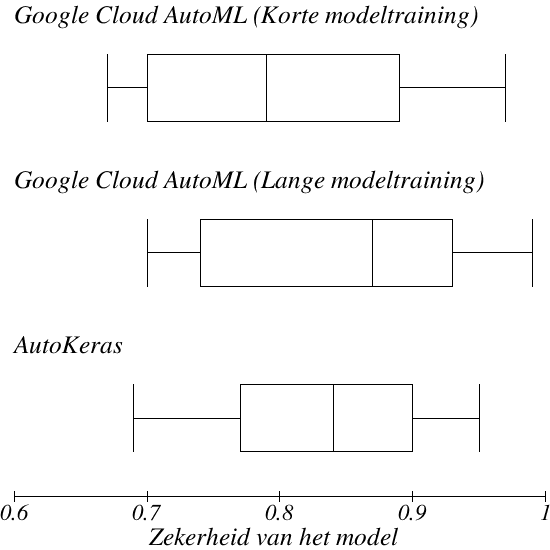
\includegraphics[width=\linewidth]{img/boxplot.png}
    \vspace{1mm}
    \caption{Verwachte correctheid van de modellen}
    \label{fig:boxplot1}
\end{figure}

Er worden goede resultaten verwacht van Google Cloud AutoML. Je betaalt voor een service en dan wil de gebruiker positieve resultaten op tafel zien. De trainingsduur van het Google Cloud AutoML model zal ook een zichtbare en positieve impact hebben op de gemiddelde score van een afbeelding. Uit het verleden hebben we geleerd dat \emph{community driven development} vaak leidt tot een performant resultaat (bv. de niet automatische versie, Keras) dat door veel developers onderhouden wordt. Voor een bedrijf is dit zeer interessant vanwege het kostenplaatje dat volledig wegvalt voor het gebruik van de technologie. 

Figuur \ref{fig:boxplot1} bevat een voorspelling van de prestaties voor de verschillende modellen.

%---------- Verwachte conclusies ----------------------------------------------
\section{Verwachte conclusies}
\label{sec:verwachte_conclusies}

AutoML zal zeker zijn plaats houden binnen het domein van machine learning. De Google Cloud AutoML interface zorgt voor een gebruiksvriendelijke omgeving waar zeer weinig programmatie aan te pas komt. Met AutoKeras moet de gebruiker meer kennis hebben van Python libraries (pandas, numpy, keras...) om tot hetzelfde resultaat te verkrijgen. 

Voor bedrijven lijkt het interessanter om voor open source te kiezen als het overeen komt met hun identiteit. Zo kunnen developers een kleine machine learning implementatie voorzien terwijl een data scientist zich kan bezig houden in grotere projecten.



%------------------------------------------------------------------------------
% Referentielijst
%------------------------------------------------------------------------------
% TODO: de gerefereerde werken moeten in BibTeX-bestand ``voorstel.bib''
% voorkomen. Gebruik JabRef om je bibliografie bij te houden en vergeet niet
% om compatibiliteit met Biber/BibLaTeX aan te zetten (File > Switch to
% BibLaTeX mode)

\phantomsection
\printbibliography[heading=bibintoc]

\end{document}
